	\documentclass[10pt]{scrartcl}

\usepackage[utf8]{inputenc}
\usepackage{tabularx}
\usepackage[ngerman]{babel}
\usepackage[automark]{scrpage2}
\usepackage{amsmath,amssymb,amstext}
%\usepackage{mathtools}
\usepackage[]{color}
\usepackage[]{enumerate}
\usepackage{graphicx}
\usepackage{lastpage}
\usepackage[perpage,para,symbol*]{footmisc}
\usepackage{listings} 
\usepackage[pdfborder={0 0 0},colorlinks=false]{hyperref}
\usepackage[numbers,square]{natbib}

\lstset{numbers=left, numberstyle=\tiny, numbersep=5pt, breaklines=true, showstringspaces=false} 

%changehere
\def\titletext{Praktikum 1 : DGL}
\def\titletextshort{Praktikum 1}
\author{André Harm}

\title{\titletext}

%changehere Datum der Übung
\date{02.11.2011}

\pagestyle{scrheadings}
%changehere
\ihead{MT, Pareigis}
\ifoot{Generiert am:\\ \today}

\cfoot{André Harms}

\ohead[]{\titletextshort}
\ofoot[]{{\thepage} / \pageref{LastPage}}

\setlength{\parindent}{0.0in}
\setlength{\parskip}{0.1in}

\begin{document}
\maketitle

\setcounter{tocdepth}{3}
\tableofcontents
\listoffigures
\lstlistoflistings


\section{Steife Differentialgleichungen}
	\subsection{Betrachtete Gleichung}
		\begin{align}
		&y(0) = 1\\
		&y' = 10 - 500 \cdot y + 5000 \cdot x
		\end{align}
		
	\subsection{Simulink/Analogrechner}
	
	\begin{figure}[htbp]
	\centering
		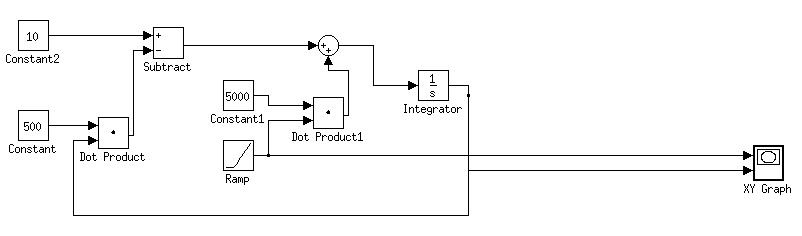
\includegraphics[scale=0.5]{simulink_aufg1_a}
	\caption{Simulink-Schaltbild: Steife DGL}
	\label{fig:simulinkAufg1}
	\end{figure}

	\subsection{Iterationsgleichungen}
		\subsubsection{Euler (expl)}
		\begin{align}
		&y_{j+1} = y_j + h \cdot ( 10 - 500 \cdot y_j + 5000 \cdot x_j )
		\end{align}				
		
		\subsubsection{Euler (impl)}
		\begin{align}
		&y_{n+1} = \frac{\frac{y_n}{h}+10+5000x_{n+1}}{500+\frac{1}{h}}
		\end{align}
		
		\subsubsection{Runge-Kutta 2}
		\begin{align}
		&k_{1_{j}} = h * (10-500y_j + 5000x_i)\\
		&k_{2_{j}} = h * (10-500y_j - 250k_{1} - 250k_{1} + 5000x_{j}+2500h)\\
		&y_{j+1} = y_j + k_2
		\end{align}			
		
	\subsection{Matlab Programme}
		\subsubsection{Euler (expl)}
			\lstinputlisting[label=code_euler_expl,caption=Explizites Euler-Verfahren, language=Matlab]{euler_expl.m}
		
		\subsubsection{Euler (impl)}
			\lstinputlisting[label=code_euler_impl,caption=Implizites Euler-Verfahren, language=Matlab]{euler_impl.m}
		
		\subsubsection{Runge\-Kutta}
			\lstinputlisting[label=code_runge_kutta,caption=Runge Kutta, language=Matlab]{rk2.m}
		
		\subsubsection{Stiff}		
			\lstinputlisting[label=code_stiff,caption=Stiff, language=Matlab]{stiff.m}		
			
	\subsection{Ergebnisausdrucke}	
		
	\subsection{Interpretation der Ergebnisse}		
		

\section{Van-der-Pol-DGL}
	\subsection{Betrachtete Gleichung}
		\begin{align}
		&y(0) = 0\\
		&\dot{y}(0) = 1\\
		&\ddot{y} = 6 \cdot (1-y^2) \cdot \dot{y} -y
		\end{align}

	\subsection{Simulink/Analogrechner}
	\begin{figure}[htbp]
	\centering
		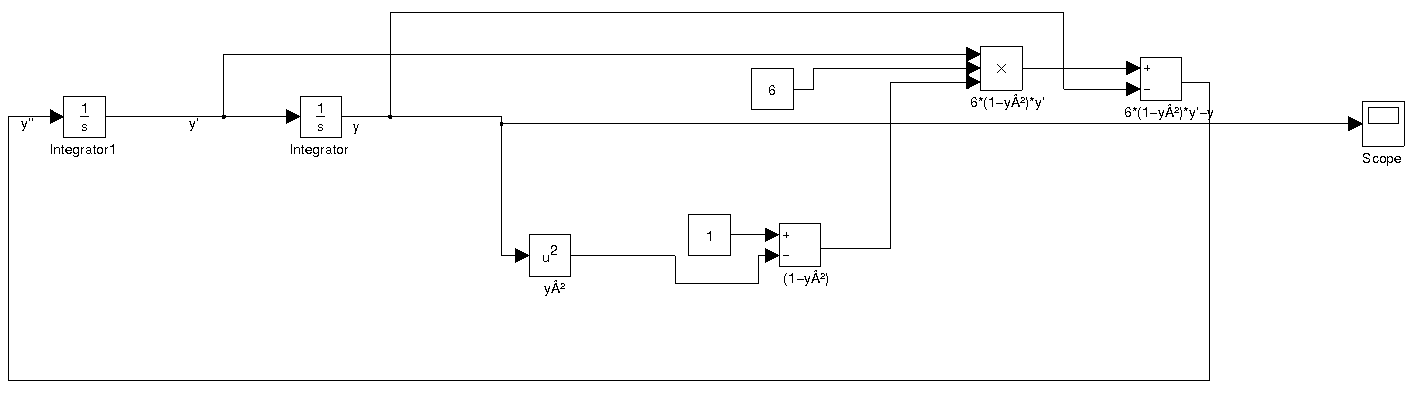
\includegraphics[scale=0.4]{aufg2_a_simulink}
	\caption{Simulink-Schaltbild: Van-der-Pol-DGL}
	\label{fig:simulinkAufg2}
	\end{figure}	
	
	\subsection{Zu DGL 1 Ordnung transformierte DGL}
		\begin{align}
		&y=z_2\\
		&y'=z_1\\
		&y''=z_1'\\
		&z_1' = 6 \cdot (1-z_2^2) \cdot z_1 - z_2\\
		&z_2' = z_1\\
		\end{align}
		
	\subsection{Iterationsgleichungen}
		\subsubsection{Euler (expl)}	
		\begin{align}
			&y_{1_{n+1}} = y_{1_n}+h*(-y_{2_n}+6*(1-y_{2_n}^{2})*y_{1_n})\\
			&y_{2_{n+1}} = y_{2_n}+h*y_{1_n}\\
			&y_{n+1} = x_{n}+h
		\end{align}
		
		\subsubsection{Runge-Kutta 2}	
		\begin{align}
			&k_{1_{y1}} = h*(-y_{2_n}+6*(1-y_{2_n}^{2})*y_{1_n})\\
			&k_{1_{y2}} = h*y_{1_n}\\
			&k_{2_{y1}} = h*\lbrace -y_{2_n} - \frac{k_{1_{y_2}}}{2} + 6 * (1-(y_{2_n}+\frac{k_{1_{y2}}}{2}^{2})*(y_{1_n}+\frac{k_{1_{y1}}}{2}))\rbrace\\			
			&k_{2_{y2}} = h*(y_{1_n}+\frac{k_{1_{y1}}}{2})\\			
			&y_{1_{n+1}} = y_{1_{n}} * k_{2_{y1}}\\
			&y_{2_{n+1}} = y_{2_{n}} * k_{2_{y2}}
		\end{align}		
	\subsection{Ergebnisausdrucke}	
		
	\subsection{Interpretation der Ergebnisse}	
	
\section{Lorenz-Attraktor mit RK 2}	
	\subsection{Simulink/Analogrechner}
	
	\subsection{Iterationsgleichungen}
		\subsubsection{Runge-Kutta 2}

	\subsection{Matlab Programme}
		\subsubsection{Lorenz}			

	\subsection{Ergebnisausdrucke}	
		
	\subsection{Interpretation der Ergebnisse}				

\end{document}

